%!TEX root = ../../main.tex

\chapter{Basics}
\section{Processing Units}
\section{RISC vs CISC}
\section{RISC-V}
RISC-V is an open standard \acf{ISA} developed by the
University of California, Berkely. The ISA is based on reduced instruction set
computer (RISC) principles. The ISA supports 32, 64 and 128 bit architectures and
includes different extensions like Multiplication, Atomic, Floating Point and more. The
ISA is open source and therefore can be used by everyone without licensing issues
and high fee requirements. Due to the open source nature of the RISC-V project,
many companies like Alibaba and NVIDIA have started to develop hardware based
on this ISA.
RISC-V opens the opportunity to optimize and configure computer hardware to a
level that would not be realizable with licensed ISA like ARM or x86. As a result of
this possibility there are many projects and companies working on hardware and
software that are beating common CPU in terms of performance and power usage
by a lot.

\section{Benchmarks}
\subsection{Coremark}
\subsection{SPECint}
\section{Memory Management}
\subsection{Memory Hierarchy}
One of the major performance factors in computing is how fast can information be accessed. Information in this case is both: data and code. Therefore high-speed infinite sized memory would be the optimum to achieve the best possible performance. Unfortunately multiple difficulties are raised by this requirement. How can an infinite sized memory be achieved, how to guarantee that access time does not increase when increasing the memory size and how to keep costs to minimum are only a few of the many questions that can be asked on this topic.\\
In general it can be said that infinite sized memory is not possible, therefore the new requirement would be: as big as possible. To achieve low access times, the memory must be placed as close as possible to the processor. The amount of extremely fast memory is therefore restricted to a finite size. Increasing the distance to the processor yields more space, hence a bigger possible memory. Access speed is reduced at the same time.\\
Therefore the only way to have a big high-speed memory is to emulate it. This is done by taking advantage of two principles: temporal- and spatial locality \cite{patterson:2017}.
Temporal locality suggests that data which is accessed will be used again in the near future. This can be caused by loops inside a routine. 
Spatial locality is very similar. If data from one particular region is accessed, there is a high probability of an access to the same region in the near future. Many data structures, for example arrays, cause spatial locality.\\
Figure \ref{fig:memHierarchy} shows an example of a possible memory hierarchy: 

\begin{figure}[h]
	\centering
	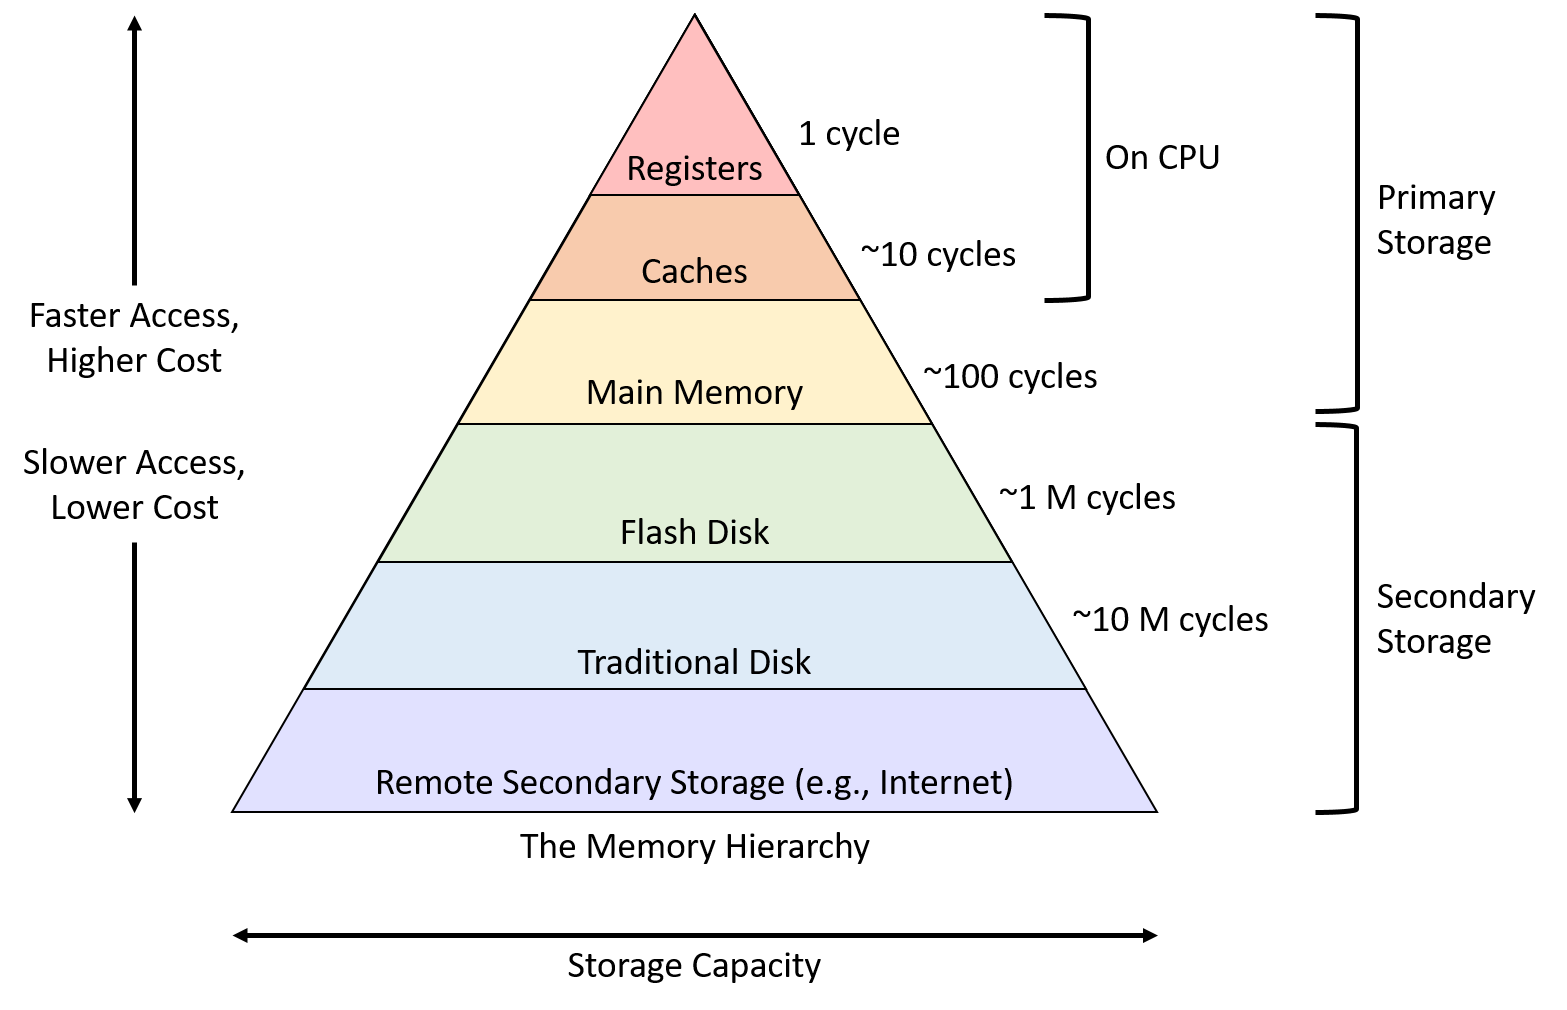
\includegraphics[width=\textwidth]{MemoryHierarchy.png}
	\caption{Generic Memory Hierarchy \cite{picture:memoryhierarchy}}
	\label{fig:memHierarchy}
\end{figure}
 
The closer a memory element is placed to the processing unit, the faster it gets. This is not only caused by the spatial distance but also by the chosen memory type. For example registers are the closest, followed by SRAM which is typically used for L1,L2 and sometimes even L3 caches \cite{patterson:2017}.\\
If a memory access is performed, the memory management system first checks whether or not the desired data is stored in the upper memory levels. A hit occurs when the data block is found in an upper level of the memory hierarchy. In case of a miss, the search for the required data block is continued in the lower levels. If it is found e.g. in main memory, the data will be provided to the processor and copied into the cache. Therefore satisfying the temporal locality principle. Surrounding data blocks are also copied to the cache in order to prevent another miss in case of spatial locality.\\
Performance of the memory hierarchy can be measured by the hit and miss rate. These describe the portion of miss and hits of the overall memory accesses. Miss rate can be calculated, if the hit rate is known:

$$miss rate = (1 - hit rate)$$

To get a significant measurement of the performance, hit time and miss penalty have to be considered as well. The hit time is defined as the time it takes to get the data block from the cache if a hit occurs. After a miss is detected, that block of data has to be retrieved from main memory, stored in the cache and provided to the processor. The overall time required for these three steps is defined as the miss penalty \cite{patterson:2017}.\\
Different ways of increasing cache performance are described in \cite{patterson:2017}.\\


\subsection{Communication Interfaces}
In order to access memory, some sort of communication interface / bus system is required. There are countless options like the widely used \ac{PCIe} and \ac{CAN} bus or application specific systems, e.g. SpaceWire used in satellite systems or \acp{ARM} \ac{AMBA}.\\
The following section will provide an overview of the \ac{AXI4-Lite} protocol which is implemented in the \ac{EDRICO}.\\
An AXI interface has four independent channels: read address, write address, read data, write data and write response. Figure \ref{fig:AXI_channels_write} and \ref{fig:AXI_channels_read} visualizes these three channels:

\begin{figure}[H]
	\centering
	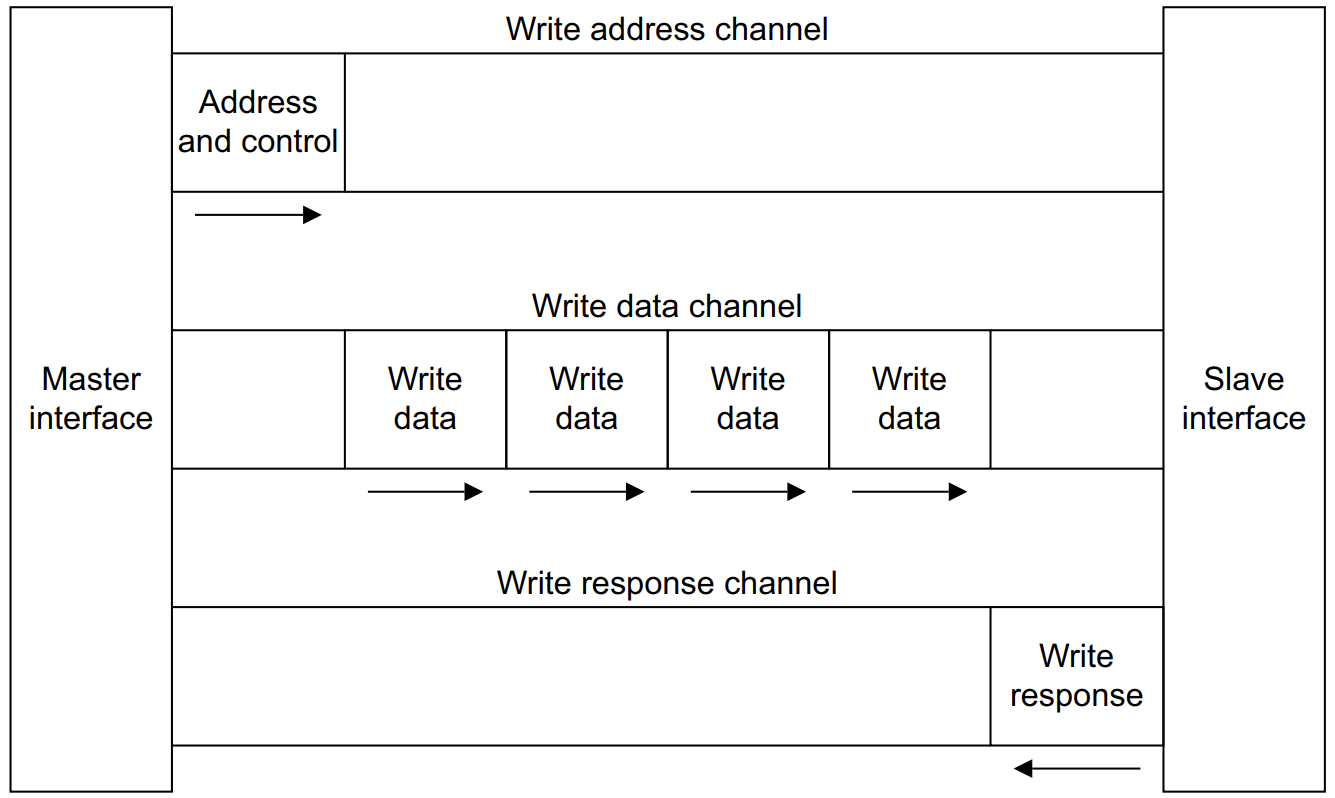
\includegraphics[width=\textwidth]{AXI4_write.png}
	\caption{\ac{AXI}4 write channels \cite{AMBA:AXI}}
	\label{fig:AXI_channels_write}
\end{figure}

\begin{figure}[H]
	\centering
	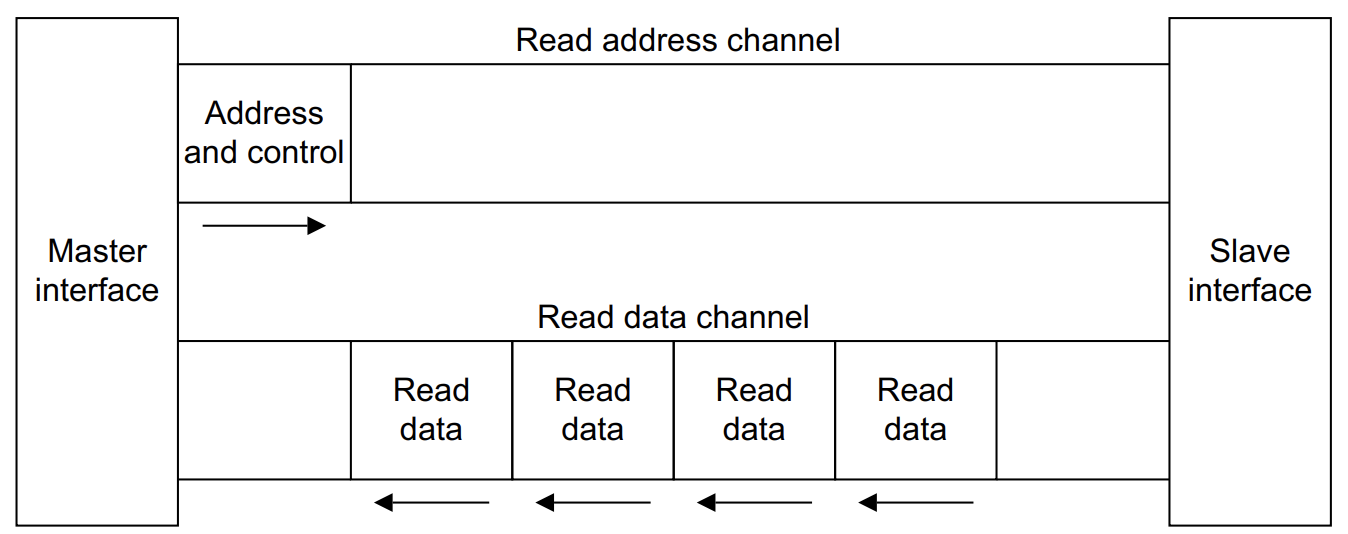
\includegraphics[width=\textwidth]{AXI4_read.png}
	\caption{\ac{AXI}4 read channels \cite{AMBA:AXI}}
	\label{fig:AXI_channels_read}
\end{figure}

The master interface always initiates the transaction by sending either the write or read address and control. In case of a write, the data is send to the slave using the write data channel. A response is given by the slave, containing information on the transfer. The slaves response on a read does not need a separate channel, since it can be transmitted using the read data channel.\\
AXI4-Lite does not support burst transfers, hence only one data word can be transmitted in one transfer. To transfer any data over any channel, a generic handshake process must be completed. Figure \ref{fig:AXI_handshake} shows how the handshake is performed:

\begin{figure}[H]
	\centering
	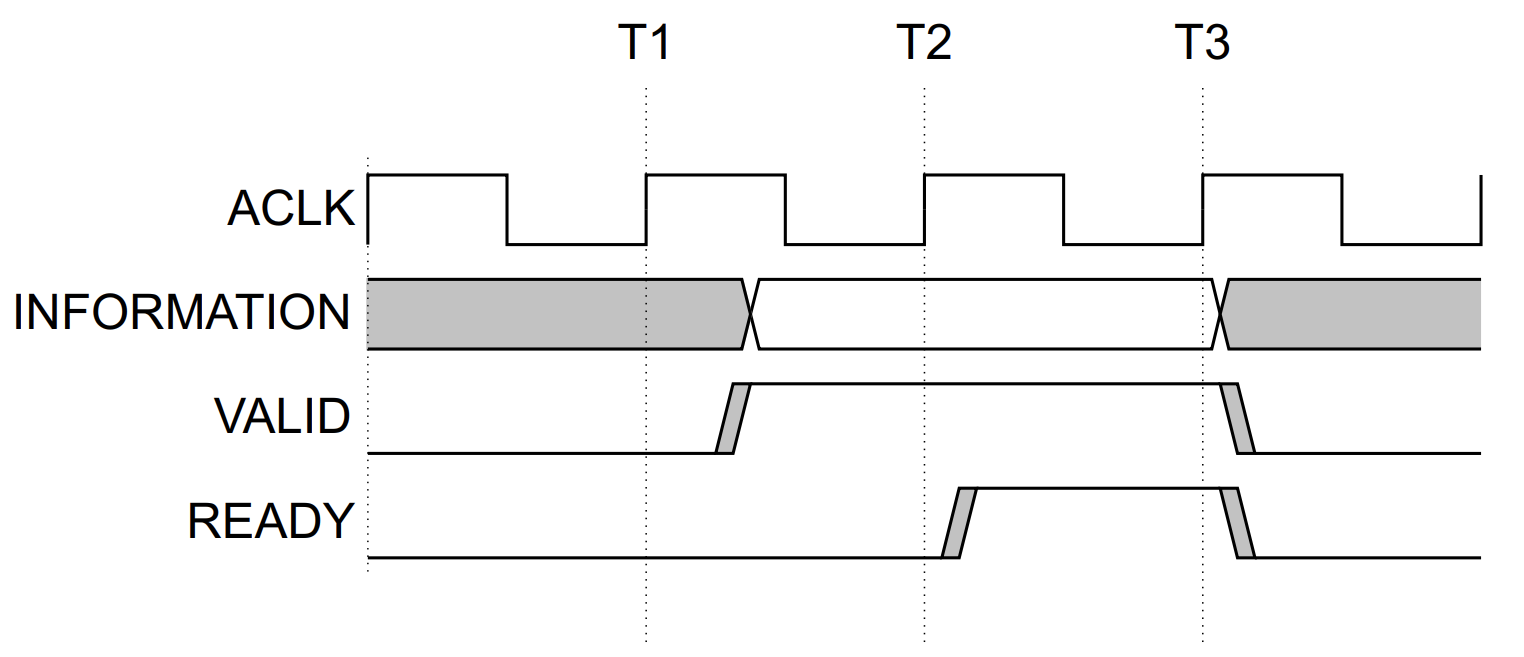
\includegraphics[width=\textwidth]{AXI_handshake.png}
	\caption{\ac{AXI} handshake \cite{AMBA:AXI}}
	\label{fig:AXI_handshake}
\end{figure}
 
At transfer begin, the sending interface applies the information (e.g. the read address) on the bus. The Valid signal indicates that the information is valid, it must stay valid until the receiving interface applies the ready signal. Ready indicates that the receiving partner is ready to receive the information. If both signals (valid and ready) are high on a rising clock edge, the information is read by the receiver and the flow control signals are tied to low \cite{AMBA:AXI}. This handshake mechanism allows the receiving \ac{AXI} interface to extend the length of the transfer when needed. Since each of the five \ac{AXI}4 channels are independent five handshake mechanisms are implemented.\\
A response of a slave contains the \textit{RRESP} or \textit{BRESP} signals, respectively. They can be set to OKAY, EXOKAY, SLVERR, and DECERR. In case of an okay or exclusive okay, no error has occurred. SLVERR indicates that an error has occurred on the slave side, even though the slave successfully registered the access. If no slave is available on the interrogated address, a DECERR is returned.\\\\
Based on the response of the slave, a masters behavior must adapt. If (EX)OKAY is returned it may proceed normal operation. If an error is detected error handling methods such as exceptions must be triggered. \\
The \ac{AMBA} protocols are widely used in embedded systems. Many \acp{IP} deployed in \acp{FPGA} can be interfaced using the \ac{AXI}4 or \ac{AXI4-Lite} bus. Therefore it is mandatory to be familiar with this particular bus architecture when working with embedded systems.




\section{FPGA}
To verify a digital circuit software simulations as well as implementing the design on
a prototype are common practice. For prototyping and even implementing a finished
product, FPGA are widely used.
FPGAs are special fine granularity Programmable Logic Devices. The digital logic
can be described using hardware description languages such as Verilog or VHDL.
These designs are then synthesized, placed and routed in order to generate a
hardware configuration file, also called bitstream. The bitstream can then be loaded
onto the FPGA via a programming interface e.g. JTAG.
Many different vendors produce FPGAs, the most famous ones are Xilinx,
Altera/Intel and Microchip. Some smaller vendors like NanoXplore produce FPGAs
targeting rare use cases like space applications.
Despite the many differences in design of an FPGA, the basic architecture always
remains the same. An array of logic cells and building blocks of different features
9 like BRAM and DSP slices are connected to each other through configurable routing
channels.
Figure \ref{fig:FPGA} shows the basic architecture of a Xilinx FPGA:\\

\begin{figure}[h]
\centering
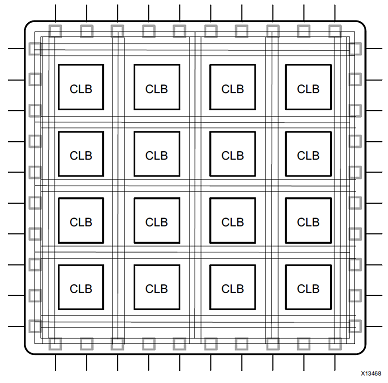
\includegraphics[scale=0.9]{fpga.png}
\caption{Xilinx FPGA \cite{xilinx:2017}}
\label{fig:FPGA}
\end{figure}

The CLBs in this architecture are comprised of LUTs and Flip-Flops, in order to implement boolean functions and allow the design of synchronous circuits. FPGAs produced by Xilinx are mostly SRAM based, other approaches are flash or anti-fuse based architectures.

\section{Hardware Description Languages}


